  \let\negmedspace\undefined
\let\negthickspace\undefined
\documentclass[journal]{IEEEtran}
\usepackage[a5paper, margin=10mm, onecolumn]{geometry}
\usepackage{lmodern} % Ensure lmodern is loaded for pdflatex
\usepackage{tfrupee} % Include tfrupee package

\setlength{\headheight}{1cm} % Set the height of the header box
\setlength{\headsep}{0mm}     % Set the distance between the header box and the top of the text

\usepackage{gvv-book}
\usepackage{gvv}
\usepackage{cite}
\usepackage{amsmath,amssymb,amsfonts,amsthm}
\usepackage{algorithmic}
\usepackage{graphicx}
\usepackage{textcomp}
\usepackage{xcolor}
\usepackage{txfonts}
\usepackage{listings}
\usepackage{enumitem}
\usepackage{mathtools}
\usepackage{gensymb}
\usepackage{comment}
\usepackage[breaklinks=true]{hyperref}
\usepackage{tkz-euclide} 
\usepackage{listings}                                      
\def\inputGnumericTable{}                                 
\usepackage[latin1]{inputenc}                                
\usepackage{color}                                            
\usepackage{array}                                            
\usepackage{longtable}
\usepackage{multicol}
\usepackage{calc}                                             
\usepackage{multirow}                                         
\usepackage{hhline}                                           
\usepackage{ifthen}                                           
\usepackage{lscape}
\begin{document}
	
	\bibliographystyle{IEEEtran}
	\vspace{3cm}
	
	\title{4.1.1.7}
	\author{EE24BTECH11059 - Y Siddhanth}
	% \maketitle
	% \newpage
	% \bigskip
	{\let\newpage\relax\maketitle}
	
	\renewcommand{\thefigure}{\theenumi}
	\renewcommand{\thetable}{\theenumi}
	\setlength{\intextsep}{10pt} % Space between text and floats
	
	
	\numberwithin{equation}{enumi}
	\numberwithin{figure}{enumi}
	\renewcommand{\thetable}{\theenumi}
	
	
\textbf{Question}:\\
Find the roots of the equation \( (x + 2)^3 = 2x (x^2 - 1) \)
\\
\textbf{Solution: }\\
First, we simplify the given equation,
\begin{align}
	x^3 -2x^2 - 6x - 8 = 0
\end{align}
We can solve the above equation using fixed point iterations. First we separate $x$, from the above equation and make an update equation of the below sort.
\begin{align}
	x = g\brak{x} \implies x_{n+1} = g\brak{x_n}
\end{align}
Applying the above update equation on our equation, we get
\begin{align}
	x_{n+1} = 	\frac{x_n^3 -2x_n^2 - 8}{6}
\end{align}
Now we take an initial value $x_0$ and iterate the above update equation. But we realize that the updated values always approach infinity for any initial value. \\
Thus we will alternatively use Newton's Method for solving equations.
\begin{align}
	x_{n+1} = x_n - \frac{f\brak{x_n}}{f^{\prime}\brak{x_n}} 
\end{align}
Where we define $f\brak{x}$ as, 
\begin{align}
	f\brak{x} = x^3 -2x^2 - 6x - 8 \\
	f^{\prime}\brak{x} = 3x^2 -4x - 6 
\end{align}
Thus, the new update equation is, 
\begin{align}
	x_{n+1} = x_n - \frac{x_n^3 -2x_n^2 - 6x_n - 8}{3x_n^2 -4x_n - 6 } 
\end{align}
Taking the initial guess as $x_0 = 1$, we can see that $x_n$ converges at the 43rd iteration with x as,
\begin{align}
	x = 4
\end{align}
Alternatively, we can use the Secant method for solving equations.
\begin{align}
	x_{n+1} = x_n + f\brak{x_n}\frac{x_{n} -  x_{n-1}}{f(x_{n}) -  f(x_{n-1})}
\end{align}
Newton's method is very powerful but has the disadvantage that the derivative may sometimes be a far more difficult expression than \(f(x)\) itself and its evaluation therefore it may be more computationally expensive. The secant's method is more computationally cheap as the equation of the derivative is avoided by taking 2 starting points.\\ 
Taking the initial guesses as $x_0 = 1, x_1 = 2$, we see that $x_n$ converges in 36 iterations with x as,
\begin{align}
	x = 4
\end{align} 
 
 Matrix Approach of solving this question: 
 If we consider the cubic equation as the characteristic equation of a matrix, then by finding the eigen-values of that matrix, we can find the roots of the equation. The matrix whose eigen-values are the roots of equation is called the companion matrix of the said equation.
 If the given polynomial is,
 \begin{align}
 	P(x) = c_0 + c_1\,x + c_2\,x^2 + \dots + c_{n-1}\,x^{n-1} + x^n
 \end{align}
 
 Then the companion matrix is given as,
 
 \begin{align}
 	M = \myvec{0 & 0 & \dots & 0 & -c_0\\1 & 0 & \dots & 0 & -c_1\\0 & 1 & \dots & 0 & -c_2\\\vdots & \vdots & \vdots & \vdots &\vdots \\0 & 0 & \dots & 1 & -c_{n-1}} \label{comp}
 \end{align}
 Applying \eqref{comp} to the question, we get
 \begin{align}
 	M = \myvec{0 & 0 & 8 \\ 1 & 0 & 6 \\ 0 & 1 & 2}
 \end{align}
 Finding the eigen-values, we get
 \begin{align}
 	x = 4 \\
  	x = -1-i \\
   	x = -1+i 
 \end{align}
 
 Matrix method for finding roots:  
 There are multiple algorithms to find the roots of a polynomial equation, but in this case, we utilize the \textbf{power iteration algorithm}. This method is particularly effective due to its simplicity and its ability to compute the largest eigenvalue of a given matrix.  
 
 The power iteration algorithm takes advantage of the companion matrix representation of the polynomial. This method leverages the fact that the roots of the polynomial correspond to the eigenvalues of the companion matrix. The steps are as follows:
 
 \begin{enumerate}
 	\item Construct the \textbf{companion matrix} for the given polynomial equation.
 	\item Use the power iteration algorithm to find the \textit{largest eigenvalue} of the companion matrix, denoted as $\lambda_{\text{max}}$.
 	\item This eigenvalue corresponds to one root of the polynomial. Remove this root from the polynomial by performing synthetic division with the factor $x - \lambda_{\text{max}}$, resulting in a new polynomial of degree one less than the original.
 	\item Repeat the above steps iteratively on the reduced polynomial until a degree-1 equation is obtained, which gives the final root directly.
 \end{enumerate}  
 
 Let the polynomial equation be:
 \begin{align}
 	P(x) = c_{0} + c_{1}x + c_{2}x^{2} + \cdots + c_{n}x^n,
 \end{align}
 where $c_0, c_1, \dots, c_n$ are the coefficients of the polynomial.  
 
 The companion matrix $C$ of the polynomial is constructed as follows:
 \[
 C = \begin{bmatrix} 
 	0 & 0 & \cdots & 0 & -\frac{c_0}{c_n} \\ 
 	1 & 0 & \cdots & 0 & -\frac{c_1}{c_n} \\ 
 	0 & 1 & \cdots & 0 & -\frac{c_2}{c_n} \\ 
 	0 & 0 & \ddots & 0 & -\frac{c_3}{c_n} \\ 
 	\vdots & \vdots & \vdots & \ddots & \vdots \\ 
 	0 & 0 & \cdots & 1 & -\frac{c_{n-1}}{c_n} 
 \end{bmatrix}.
 \]
 
 The power iteration algorithm computes the largest eigenvalue $\lambda_{\text{max}}$ of this matrix by iteratively applying the following steps:
 \begin{align}
 	\mathbf{x}_{n} &= C \mathbf{x}_{n-1}, \\
 	\mathbf{x}_{n} &= \frac{\mathbf{x}_{n}}{\|\mathbf{x}_{n}\|},
 \end{align}
 The iteration stops when:
 \begin{align}
 	|\lambda_{\text{max}}^{(n)} - \lambda_{\text{max}}^{(n-1)}| < \epsilon,
 \end{align}
 where $\epsilon$ is the desired precision, and $\lambda_{n} = \frac{\mathbf{x}_{n}^\top C \mathbf{x}_{n}}{\mathbf{x}_{n}^\top \mathbf{x}_{n}}$.  
 
 Once $\lambda_{\text{max}}$ is found, synthetic division is performed to reduce the polynomial:
 \begin{align}
 	P(x) &= P(x) \div (x - \lambda_{\text{max}}), \\
 	P(x) &= c_{1,0} + c_{1,1}x + c_{1,2}x^{2} + \cdots + c_{1,(n-1)}x^{n-1}.
 \end{align}
 Now, the new companion matrix will be evaluated.  
 
 This process is repeated iteratively until the polynomial is reduced to a degree-1 equation:
 \begin{align}
 	P_1(x) = c_{n-1,0} + c_{n-1,1}x.
 \end{align}
 Thus, the effective update equation would be:
 \begin{align}
 	P_{n-1}(x) &= P_{n}(x) \div (x - \lambda_{n}),
 \end{align}
 where $\lambda_{n}$ can be found using the power iteration of the companion matrix of $P_{n}(x)$.  
 
 Complexity Analysis:  
 
 The time complexity of this method is dominated by:
 \begin{itemize}
 	\item The construction of the companion matrix: $O(n^2)$.
 	\item The power iteration process: $O(k \cdot n^2)$, where $k$ is the number of iterations required for convergence.
 	\item Synthetic division: $O(n)$.
 \end{itemize}
 
 Across all roots, the overall time complexity is approximately:
 \begin{align}
 	O(n^3),
 \end{align}
 which is typical for eigenvalue-based methods. \\
Results: For a 5th-degree equation with real roots, this algorithm took 1.3 ms compared to the standard LAPACKE eigenvalue solver (Givens Rotations), which took 2.4 ms. An optimized Givens Rotation eigenvalue finder can compute the eigenvalue for the tested matrix in 0.94 ms.

	\begin{figure}[h!]
		\centering
		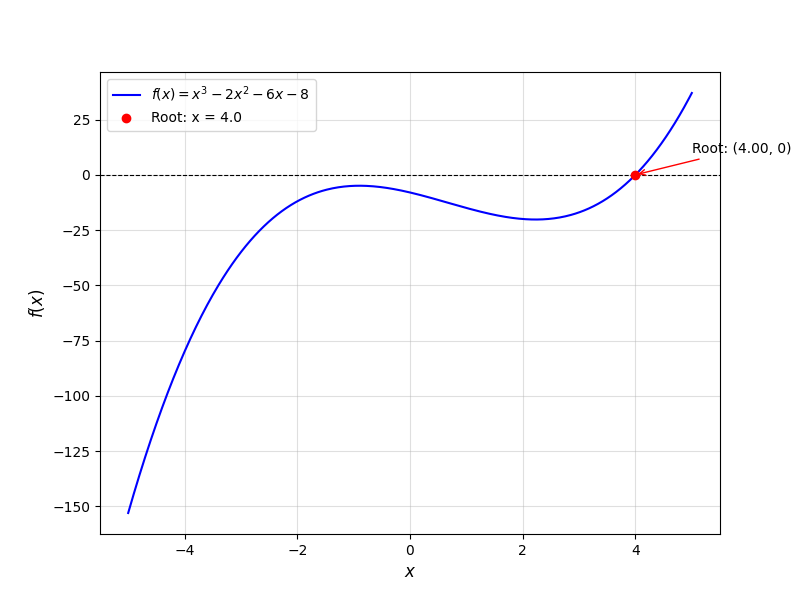
\includegraphics[width=\columnwidth]{figs/fig1.png}
		\caption{Solution of the given function}
		\label{stemplot}
	\end{figure}
	
	
\end{document}  